\section{Design Options for Secure Virtualization Systems}
\label{sec.design}

%Many security systems for protecting privileged code have been proposed and
%developed over the years. The challenge for all of these systems is how to
%balance security and functionality for applications. In this section, we explore previous approaches to
%dealing with this safety/usability trade-off.

Providing essential system functionality without exposing privileged code is one of the
primary challenges. %facing designers of secure virtualization systems.
Currently, there are two basic approaches.
One, called ``System Call Interposition (SCI)," checks and passes system calls
through to the underlying kernel. The other, known as ``functionality
reimplementation," requires rebuilding system functionality with new code. In the
following, we show that both methods are limited in their ability to
prevent attacks in the kernel. %After examining the key ideas in both approaches,
With our metric in Section~\ref{sec.metric}, 
we propose a new design scheme named ``Lock-in-Pop" that combines safer reimplementation
within a secure environment, and accesses only popular code requests through a
very small trusted computer base.

%from triggering and exploiting vulnerabilities

%but taking it a step further,
%that

\subsection{System Call Interposition (SCI)}
SCI is the long-standing idea behind sandboxing systems like Janus
\cite{Janus0:96, Janus:99}. It relies on the underlying kernel
to provide system functionality. To prevent attackers from undermining the system,
SCI uses a system call filter module to mediate requests
from untrusted user code instead of allowing it to go directly to the kernel.
The filter will check a predefined security policy to decide which system calls are
allowed to pass to the underlying kernel, and which ones must be stopped.
%The security policy usually
%can be defined by the system administrator through a policy engine.
%
Figure \ref{fig:design_system_call_interposition} illustrates the general design
of a system call interposition system.

\begin{figure}%[h]
\centering
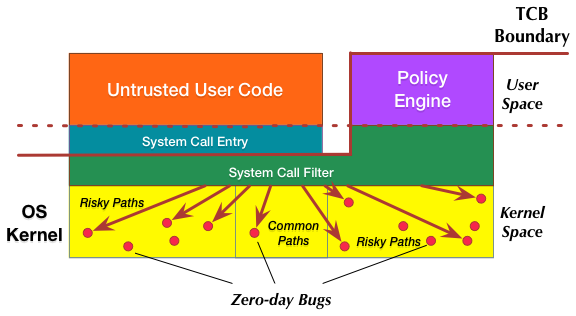
\includegraphics[width=1.0\columnwidth]{diagram/Virtualization_Design_Model_03.png}
\caption{\small Schematic of System Call Interposition.}
\label{fig:design_system_call_interposition}
\end{figure}  \lois{Yiwen, remember to address Yanyan's comment here about the placement
of the TCB boundary in Figure 2 being above the uaer space}

System call interposition was once a popular approach to the design of secure
virtualization systems because it gave developers the power to set and enforce
security policies. \lois{I think I asked this during the ;last revision. You say "was"
a popular approach. Is it not a popular approach anymore?}
%that could pass or stop a system call in a straightforward way.
However, this design
is limited by its overly complicated approach to policy decisions and implementation.
To make a policy decision, the system needs to
obtain and interpret the OS state associated with the programs it is monitoring.
\lois{Can you clarify the above sentence? What do you mean by the OS state?} The
complexity of OS states makes this process difficult and can lead to
inaccurate policy decisions.
Second, there are many indirect paths in the kernel that can be accessed.
Overlooking those paths would render the
system call interposition policy ineffective, because attackers will be able to
bypass the imposed security checks.\lois{Who or what is "overlooking those paths"}
Moreover, many side-effects of blocking
certain system calls could affect the function of desired system calls.
It is difficult for developers to fully understand the side-effects of all the
system calls in an interface as complex as the UNIX API. \lois{can you either
define or give an example of these "side-effects"} This makes
it challenging to design and build a secure virtualization system using
system call interposition alone.
%Eventually, developers turned to the idea of
%reimplementation, which is more practical.

\subsection{Functionality Reimplementation}
%Since using system call interposition alone does not offer sufficient protection,
%%to serve the purpose of
%%a modern system, where complex and risky system functionality is required,
%virtualization system designer have begun creating their own system
%interface and library. 
Systems such as  Drawbridge \cite{Drawbridge-11},
 Bascule \cite{Bascule}, and Graphene \cite{Graphene-14} can
provide richer functionality and run complex programs than most systems built
with SCI alone. These systems have their own system
interfaces and libraries. Some virtualization
systems, such as OS VM systems VirtualBox, and VMWare Workstation, even have the
full functionality of an OS reimplemented in their codebase. We call such a design
``functionality reimplementation."

\begin{figure}%[h]
\centering
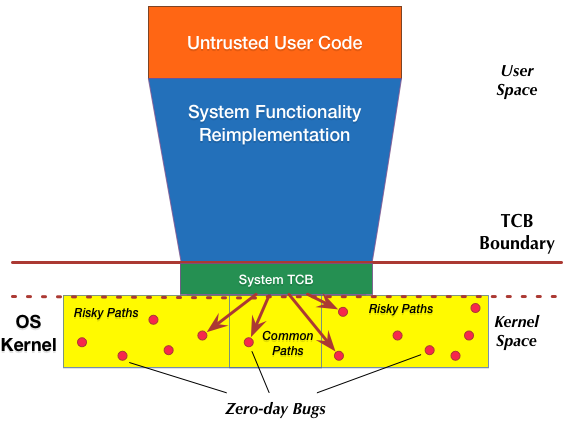
\includegraphics[width=1.0\columnwidth]{diagram/Virtualization_Design_Model_02.png}
\caption{\small Schematic of Functionality reimplementation System.}
\label{fig:design_functionality_reimplementation}
\end{figure}

The key idea of this design is to not fully rely on the underlying
kernel for system functions. Instead, critical OS functions are re-written with new
code. As illustrated in Figure \ref{fig:design_functionality_reimplementation},
 this design scheme reimplements its own system functionality to provide to user code.
\lois{Please check the previous sentence. I re-wrote it because it was a bit awkward,
 but I may have changed the meaning} When it has to communicate with the kernel
to access resources like memory, CPU, and disk storage, the system will do so with
its underlying TCB code, which can access the kernel directly.
For example, Graphene \cite{Graphene-14} reimplements
its own Linux system calls in the
\texttt{libLinux.so} module. When it needs to acquire resources from
the kernel, it uses a
Platform Adaptation Layer (PAL)  module that has access to the kernel
and provides basic ABI functions to the OS library.

Functionality reimplementation provides a more realistic solution to building
virtualization systems than earlier efforts, and offers rich functionality.
However, hundreds of vulnerabilities in existing virtualization systems have still been
reported ~\cite{NVD}.\lois{Do we have a time frame here? Over what period of time were
those vulnerabilities reported} One shortcoming of such a system is the size
of the implementated components. To provide rich functions, systems using this design have
introduced larger codebases and increased the size of their TCBs. In addition, the
complexity of OS functions can easily result in bugs and vulnerabilities in
reimplementation \lois{Complexity in what sense?}. Some vulnerabilities
will directly cause a privilege escalation, which allows attackers to escape the sandbox
and execute arbitrary code on the host OS. \yanyan{give an example.}
%is not as secure as people have thought and


%Besides these severe vulnerabilities that can lead to attackers taking direct control
%of the machine,
Even operations that are considered
legal and harmless in the guest OS may open up system call paths into the underlying
host OS and cause a problem.
The second type of problem\lois{What does the "second type" refer to?} can be fatal,
as it can reach and trigger vulnerabilities in the underlying OS kernel.

%Problems with the existing functionality reimplementation design indicate that there
%is a lot more to do to build secure virtualization systems. The next step was to
%combine the strengths of both systems and the guidance of our metric to explore a
%new design template.

\subsection{Lock-in-Pop: Staying on the Beaten Path }
A common weakness of both of these previous approaches is the inevitable contact
between the privileged code of the kernel and the untrusted application. 
By leveraging our key observation
 that ``popular, frequently-used kernel paths contain fewer bugs" we propose a design
in which all code \emph{including the complex part
of the operating system interface} should access only
popular kernel paths through a small TCB. As it ``locks" all functionality
 requests into only the ``popular" paths, we thus dubbed the
design ``Lock-in-Pop."

In addition, the system is entirely in the userspace, and both the size of
 the sandbox kernel and its access to the OS kernel is restricted
(Figure \ref{fig:design_safe_reimplementation}). Any complex or possibly risky system
functions that require contact with the OS kernel is reimplemented using
memory-safe code and is contained within a sandbox. This approach has advantages
over the others that require modifications to
the OS kernel (Section {\ref{sec.metric}). The isolation provided by placing
Lock-in-Pop in the userspace is also an added protection over functionality
reimplemention. If a modified module is in the OS kernel and is compromised, it
exposes kernel privileges that could allow attacks 
in the underlying system and any applications in the userspace.

%In this manner, any bugs
%or failures within the implementation of these complex system functions
%are contained by the sandbox.
%as it avoids the risk of threat escalation.

As shown in Figure \ref{fig:design_safe_reimplementation}, the Lock-in-Pop design
has two components. The first is a computational module that enables the system to
support and run legacy applications, and execute binary code compiled from unmodified
source code on popular hardware architecture. This module's main responsibility is
to provide an execution environment that can run unmodified source code. It also
performs functions like type checking, object creation, and garbage collection.
\yanyan{I don't see the computational module in the figure.}
The second is a library OS that serves requests to access the OS kernel.
\yanyan{why in the figure it's called "library OS sandbox"?}
The system invokes the computation module to perform its operations,
and, if there are riskier calls, the computation module directs those requests to the
library OS.

In turn, the library OS responds to the system call requests and
returns results to the user code, if the requests are granted.
It is comprised of two parts: a sandbox kernel that provides access to basic but critical
system calls, and a system API safe reimplementation that implements more
complex calls, such as file system calls. \yanyan{in the figure it's called
"system functionality safe reimplementation".}
%
The sandbox kernel forms the only TCB of our library OS, and is kept
extremely small and simple so that it is easy to verify its security.
The sandbox code provides an API that performs a few critical system calls with
the most basic parameters, such as writing data to the file system
and communicating with the network. The kernel utilizes the most simplistic calls
possible with the most basic arguments. \yanyan{this paragrah talks about
sandbox kernel, but never metioned safe reimplementation.}

\begin{figure}%[h]
\centering
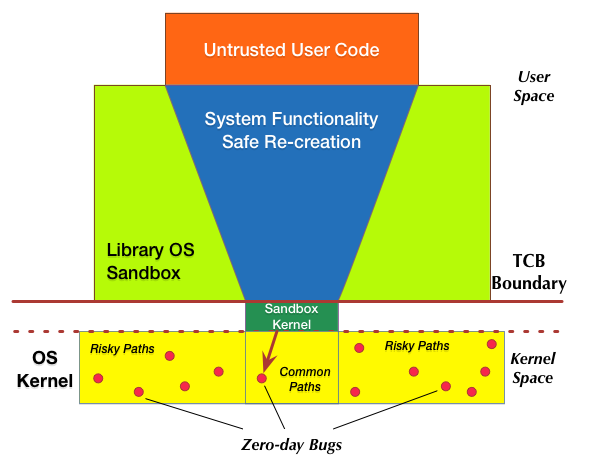
\includegraphics[width=1.0\columnwidth]{diagram/Virtualization_Design_Model_01.png}
\caption{\small ``Lock-in-Pop''System ensures safe execution of untrusted user code
despite existing potential zero-day bugs in the OS kernel.}
\label{fig:design_safe_reimplementation}
\end{figure}


%\subsubsection{The Computation Module}
%
%Providing an execution environment that can run unmodified source code is
%the main responsibility of the computation module. The key security issue of executing system calls
%without triggering OS kernel bugs is left to the library OS module.



%It should have a set of capabilities that enable the construction of essential and more complicated functions.
%For example, the sandbox kernel capabilities should include basic functions for network,
%file system I/O, lock, thread, and namespace. It also needs to have access to the OS kernel through system calls.
%In developing our design, we leveraged our verified hypothesis that commonly used kernel paths contain fewer bugs.
%Thus, the system calls we allow in our sandbox kernel are common calls, like file open, read, write, and close.
%Furthermore, the set of arguments used for each call is also highly restricted.

With the computation module and the library OS module, unmodified user code is able to run on top of our designed system.
It is important to note that our design does not rely on any specific technique or tool, and it is possible
to choose from several different techniques that fit specific security requirements.
The following section describes one implementation of our design called Lind.

%Based on this general system, we implemented a prototype security system based on a controlled kernel access that we called Lind.
%Below we offer a short explanation of one design feature: the use of dual sandboxes.
%The following section offers a more detailed description of Lind's design and implementation.
%
%\subsection{The Roles of the Dual Sandboxes}
%
%In reviewing our design, some fundamental questions could be raised about the dual sandbox design choice.
%"Why is one not enough?"" And, "If two is good, why not use three or more?""
%The answer to the first question is that the kernel interface is extremely rich and hard to protect.
%In order to have minimal impact on the kernel, as well as provide sufficient API for legacy applications,
%we need to have one sandbox focuses on protecting the kernel and providing POSIX API.
%With two sandboxes, one serves as the computation module,
%while the other one is the library OS module. As to the second question,
%which could be rephrased as ``why not sandbox the sandbox kernel TCB and get more security?,''
%the lowest level sandbox eventually must have some fundamental,
%even if limited, access to system resources, such as memory, and storage, threads.
%So even if we were to sandbox the sandbox kernel and have additional sandboxes,
%the one at the bottom level will still access the OS kernel in a similar way.
%Thus, having multiple sandboxes does not provide any extra security benefits.
%\yanyan{it's better to tie in with earlier paragraphs and talk about why we need
%computation + lib OS. we normally don't do Q\&A like this.}
